% vim:ft=tex:
%
\documentclass[12pt]{article}
\usepackage{natbib}
\usepackage{graphicx}
\usepackage{url}

\title{
	Clustering of Cross-Referenced Astronomical Data Sets
}
\author{
	Vera Abaimova --- \texttt{stormseecker@gmail.com} \\ 
        Mark Wells --- \texttt{mwellsa@gmail.com}
}

\date{December 9, 2014}
\begin{document}
\maketitle

\begin{abstract}
The large amount of astronomical data that is now available from a multitude of missions creates a need for machine learning methods that can analyze it and glean information about our universe.
One challenge in particular is to analyze data about the same observations made by different missions, \textit{i.e.}, analyze cross-referenced data, especially data in different formats.
One such format is time series data provided by the \textit{Kepler} mission, which results in additional difficulties.
Our proposed method extracts features from cross-referenced data sets, including time series data, and applies a hierarchical clustering model in order to aid stellar classification.

\end{abstract}

\section{Introduction} % (fold)
\label{sec:Introduction}

\subsection{Motivation} % (fold)
\label{sub:Motivation}
Astronomy and astrophysics is a constantly growing field that is heavily data-dependent. 
In the near future, petabytes of data will be procured on any given night by the various telescopes and scientific missions tasked with surveying the night sky in the search for objects of interest.
Such a large quantity of data means that there is a dire need for quick object identification and classification in order to obtain useful knowledge from the data, a task that has quickly grown beyond the ability of unaided humans.

The introduction of machine learning into the field of astrophysics has resulted in a new discipline that combines the two areas of research: astroinformatics.
The goal of astroinformatics is to harness the power of machine learning and data mining in order to find new and interesting knowledge from the stockpile of data that is constantly being produced at an accelerated rate.

The numerous astronomical surveys currently in operation often times (and not by accident) generate data on overlapping parts of the sky.
Each mission generates different types of information: spectral, spatial, temporal, or any combination.
The result is that some of the same stars will appear in multiple data sets and will have more diverse data available via the contribution of the different missions.
Unfortunately, not a lot has been done with this synergy, as most of the current literature indicates that the majority of effort goes to classifying stars using one data set alone.
However, there are a few efforts out there that maximize their study by combining data from multiple (and varied) data sets.

Ultimately, the acquisition of data and its interpretation into interesting information will help humanity better understand the universe in which we live.
% subsection Motivation (end)


\subsection{Challenges} % (fold)
\label{sub:Challenges}
There are numerous challenges that arise when trying to correlate different astronomical data sets.
Routinely, the data is in different forms and of different resolutions.
Sometimes there is target confusion which makes it difficult to separate the received signal from two or more potential sources.
For example, there could exist a background star and its variability could be falsely detected when measuring the foreground star of interest.

Other factors also serve to compound this already difficult process.
Missing data is very common: the spacecraft had to slew to a transient event, the post-processing performed by the mission team had to truncate data, or the object was too faint to be observed.
Since these factors are spacecraft dependent it is quite possible that even when two stars are in both data sets, pertinent data could be missing from one of the sets which would exclude its utility.

When it comes to analyzing the data it is sometimes difficult to correlate the separate features in a useful way.
Obviously the location of an object in the sky seldom has any relevance (save in certain unique cases).
Also, bias could be an issue.
Stars, because of their inherent properties, could be excluded from one dataset but not another, so entire classes of objects are underrepresented.
With analysis of time series data, the sheer size of the data presents challenges.
It is difficult to work directly with all of the data points in such a format.
How we mitigated this problem is further discussed in Section~\ref{sec:Method}.

Finally, the sheer amount of data available and even the data set that we ended up working with is incredibly large so it took a long time to process and it was computationally expensive to analyze.
% subsection Challenges (end)


\subsection{Related work overview} % (fold)
\label{sub:Related work overview}
In the existing literature there are several data mining approaches that are employed when analyzing astrophysical and astronomical data. 
These fall into the following camps: supervised learning, unsupervised learning, and semi-supervised learning. 
We will only be concerning ourselves with unsupervised learning, specifically clustering, and we will also take a look at distributed data mining.

Clustering is an extremely popular unsupervised method in the field of astrophysics.
Distributed data mining is an approach that is useful for, but not limited to, large data sets. 
All of these methods will be discussed in further detail as part of the related work in current literature.
% subsection Related work overview (end)


\subsection{Proposed Method} % (fold)
\label{sub:Proposed Method}
Our proposed method consists of cross referencing three data sets: \textit{Kepler}, \textit{GALEX}, and \textit{SDSS} and then extracting the relevant features.
The \textit{Kepler} data set also provides time series data, so part of the feature acquisition process involved processing the time series lightcurves and extracting useful features from them.
Before we could do that though, we performed a process called flattening, which we did twice, once over each quarter and again over each day of data.
After the flattening process we extracted the variance, skewness, and kurtosis of each lightcurve and included the resulting values in our feature space.

After the data preprocessing we performed an analysis.
Our chosen baseline method is hierarchical clustering, which performed better than the K-Means clustering we performed for our preliminary data analysis. 
More in depth explanations of both our methods and experimental results are further outlined in Section~\ref{sec:Method} and Section~\ref{sec:Experiments}, respectively.
% subsection Proposed Method (end)


\subsection{Overview} % (fold)
\label{sub:Overview}
In Section~\ref{sec:Related Work} we will give a short survey of the literature which outlines existing approaches to processing time series data and working with large data sets.
The next section, Section~\ref{sec:Problem Definition} will include a formal, mathematical definition of our problem, including the input and the expected output.
Section~\ref{sec:Method} is where we will go more in depth about our process, first about the baseline methods we tried in our preliminary analysis of the data, and then about our final data analysis.
Section~\ref{sec:Experiments} will contain information about our data sets, our experimental results, both for our preliminary and final passes, and an analysis of our final results.
The final section is a summary of the problem and our experimental results, along with what we have learned from this project.
% subsection Overview (end)

% section Introduction (end)

\section{Related Work} % (fold)
\label{sec:Related Work}
Clustering is an unsupervised method of machine learning, which means that one of its inherent advantages is that it does not require ground truth labels.
This is helpful in astrophysics, where most of the data is unclassified (at least initially) and thus does not have available labels to train the model.

One instance where this is useful is in the study of time series data, as described by \cite{wang}.
There are a variety of time series clustering algorithms, all of which are fairly effective at dealing with moderate-length time series.
There are some drawbacks, however.
Hierarchical clustering, for example, is one of the most widely used approaches, but it is limited to small time series data sets.
K-means is faster than hierarchical, but it is impractical since the clusters have to be preassigned.
Missing values can also be problematic when dealing with time series data \citep{wang}. 

The greatest advantage of clustering is that it can handle incredibly large data sets \citep{januzaj}.
An interesting improvement on the different clustering methods would be to apply them to small subsets of data and then combining the results. 
This would be an example of an application of distributed data mining.

Traditional data mining analysis is performed on data in a single set.
The advantage of distributed data mining is that data can be gathered from multiple data sets \citep{McConnell}.
This includes multiple data sets with different feature spaces.

Distributed data mining can handle large data sets very well, but an additional advantage is that it deals effectively with privacy concerns stemming from attempting to integrate all data into a central location. Furthermore, integrating large data sets together is computationally expensive, so distributed methods are ideal for these situations as described by \cite{McConnell2}. 

Distributed data mining combines several data sets to improve prediction models. 

% section Related Work (end)

\section{Problem Definition} % (fold)
\label{sec:Problem Definition}

% Some of the below values are now different thanks to our additional work

The input of our clustering problem is a list of $x_i,_j$ where $x_i$ is the star object, numbered from 1 to 20,840 and $j$ is the feature, numbered from 1 to 29.
Our feature space includes features such as $fuv\_mag$, $nuv\_mag$, and $kepmag$, among others, where $fuv\_mag$ is the far ultraviolet magnitude, $nuv\_mag$ is the near ultraviolet magnitude, and $kepmag$ is a measure of brightness of an object in the \textit{Kepler} pass band.

Our output is a list of $x_i,_j \in C_k$ where $C$ is cluster and $k$ denotes cluster number. 

% section Problem Definition (end)


\section{Method} % (fold)
\label{sec:Method}
\subsection{Preprocessing}
\label{sub:Preprocessing}
Our data from the \textit{Kepler} spacecraft is stored in \textit{FITS} files (Flexible Image Transport System).
These files can contain \emph{headers} and \emph{tables}.
We also obtained data from the \textit{Galex} mission.
All of this data was processed using \emph{Julia} (\url{http://julialang.org/}).
In order to expedite the preprocessing we broke up the dataset and distributed it over several systems.

\subsubsection{Header Information}
\label{ssub:Header Information}
For our data set the headers will contain some physical properties that we will be interested in using and the tables will contain the time series data.
These keywords, shown in Table~\ref{tab:keywords}, are provided by the \textit{Kepler} team.
These files provided values such as the stellar radius, metallicity, effective temperature, and the like.
Furthermore, these files, which came from \textit{Kepler}, also contained some information from the \textit{SDSS} mission.
The features that come from this mission include a variety of band magnitudes and color bands.

\begin{table}
    \begin{center}
    \begin{tabular}{|c|}
        \hline
        KEPLERID\\
        GMAG\\
        RMAG\\
        IMAG\\
        ZMAG\\
        D51MAG\\
        JMAG\\
        HMAG\\
        KMAG\\
        KEPMAG\\
        GRCOLOR\\
        JKCOLOR\\
        GKCOLOR\\
        TEFF\\
        LOGG\\
        FEH\\
        EBMINUSV\\
        AV\\
        RADIUS\\
        \hline
    \end{tabular}
    \end{center}
    \caption{A list of the keywords that were extracted from the headers of the FITS files.}
    \label{tab:keywords}
\end{table}

\subsubsection{Time Series}
\label{ssub:Time Series}

A single FITS file will contain the lightcurve of one quarter.
A quarter is one season, i.e. three months.
This file breakup is because the spacecraft will have to rotate itself to keep its solar panels directed toward the sun.
This means that for one star we will can have as many as 16~separate files that will need to be stitched together, resulting in a total of 349,424 files.
The time series data consists of two separate vectors: time and flux.

The flux mean level will be different for each quarter, so when we stitched the lightcurves together, we removed the mean level from each quarter.
We refer to this process as a Quarterly-Flat.
We repeated the process, only this time removing the mean from the lightcurves by day, performing a novel process called a Daily-Flat.
We then extracted the variance, kurtosis, and skewness of each type of flatted lightcurve.
The benefits of performing the flattening process is that it attenuates signals with periods greater than a day from the lightcurves.

\begin{figure}
    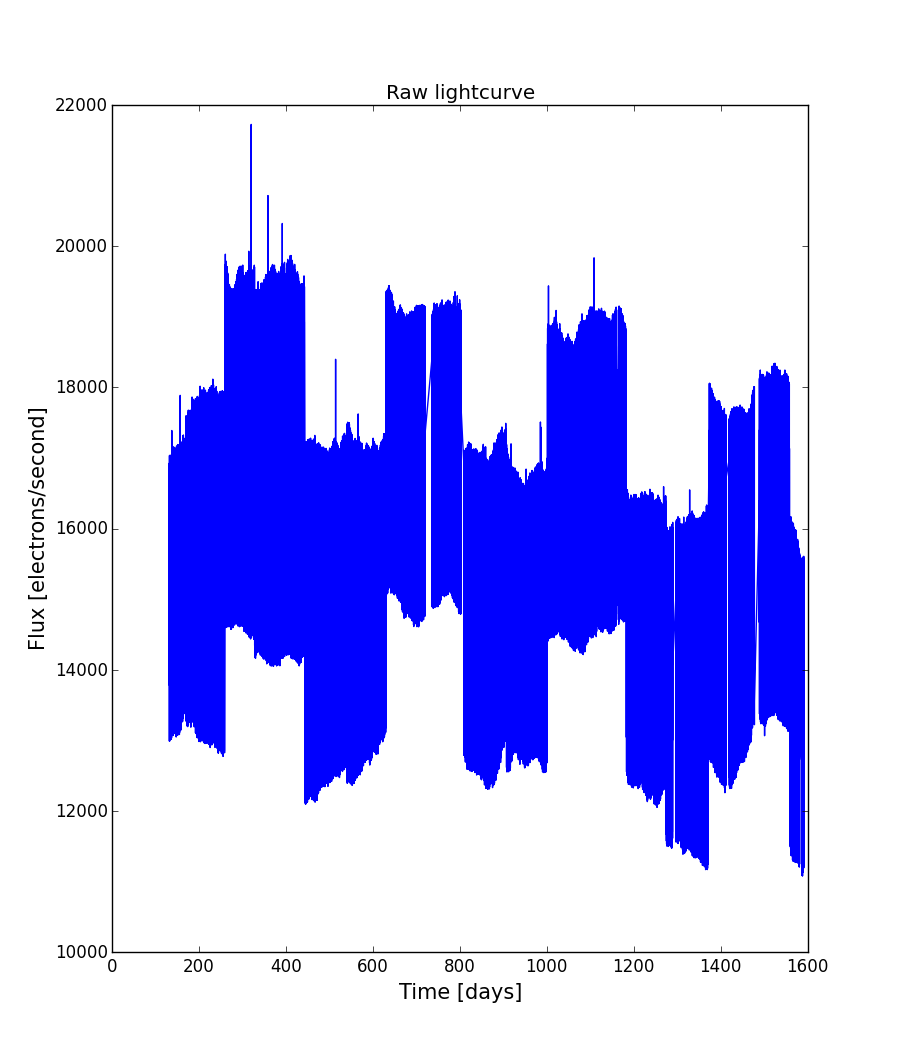
\includegraphics[width=\textwidth]{Raw_lightcurve.png}
    \caption{The lightcurve once it has been stitched together.}
    \label{fig:Raw_lc}
    
\end{figure}

\begin{figure}
    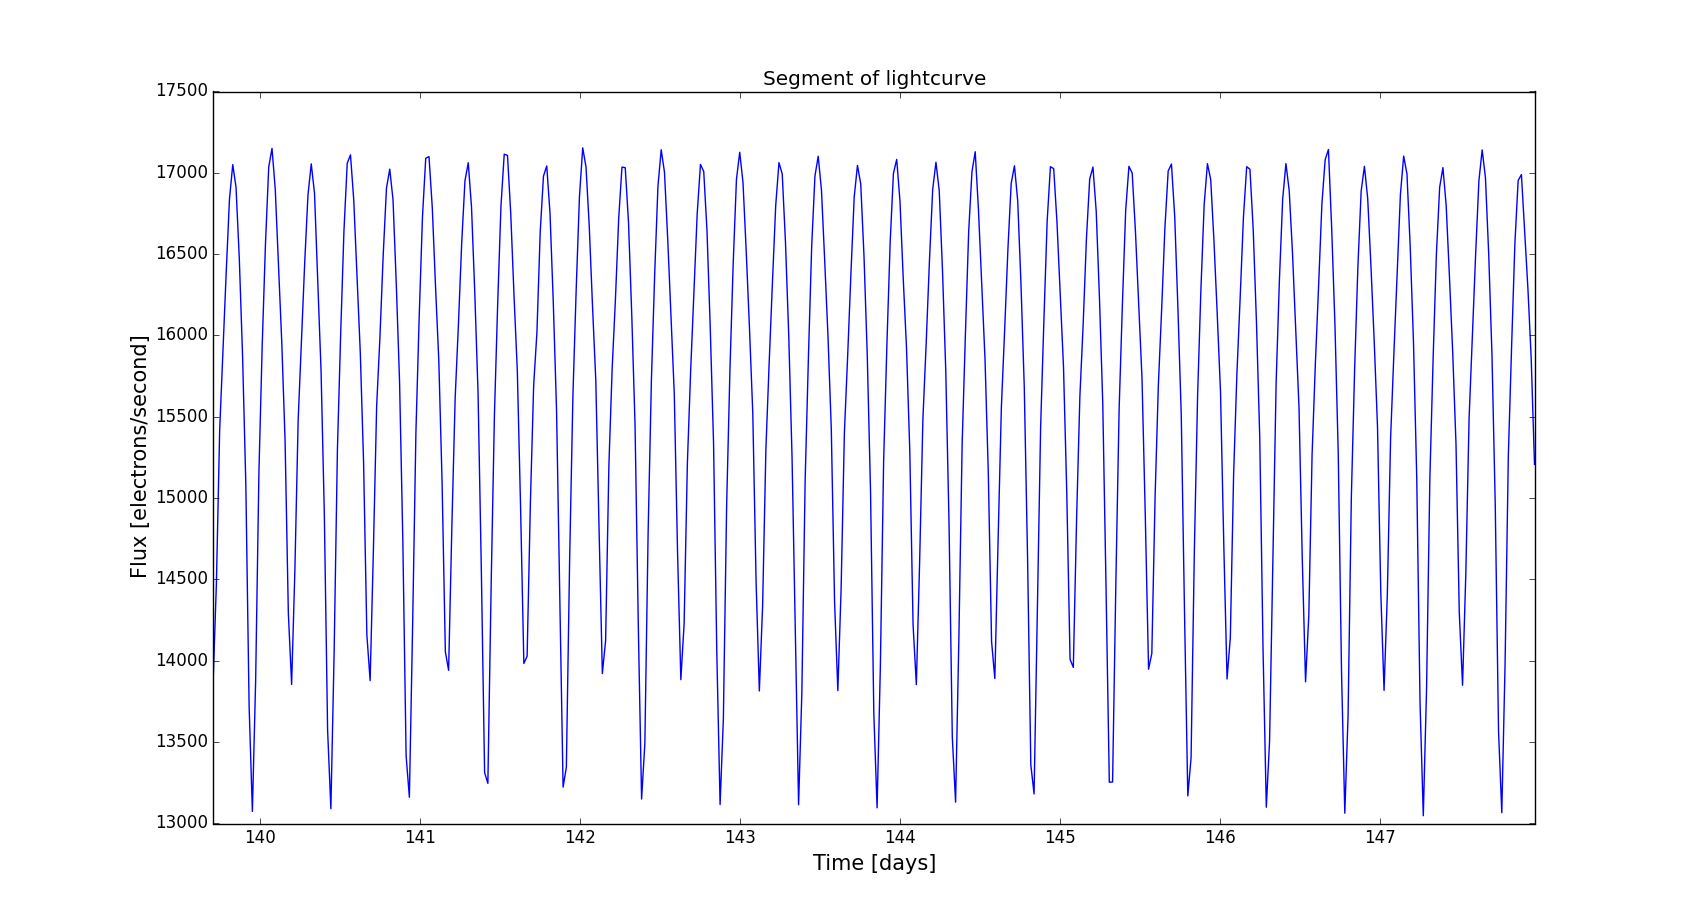
\includegraphics[width=\textwidth]{Segment_of_lightcurve.png}
    \caption{An 8.26 day segment of a raw lightcurve, meant to illustrate the inherent structure that is difficult to see in Figure~\ref{fig:Raw_lc}.}
    \label{fig:Seg_lc}
    
\end{figure}

\begin{figure}
    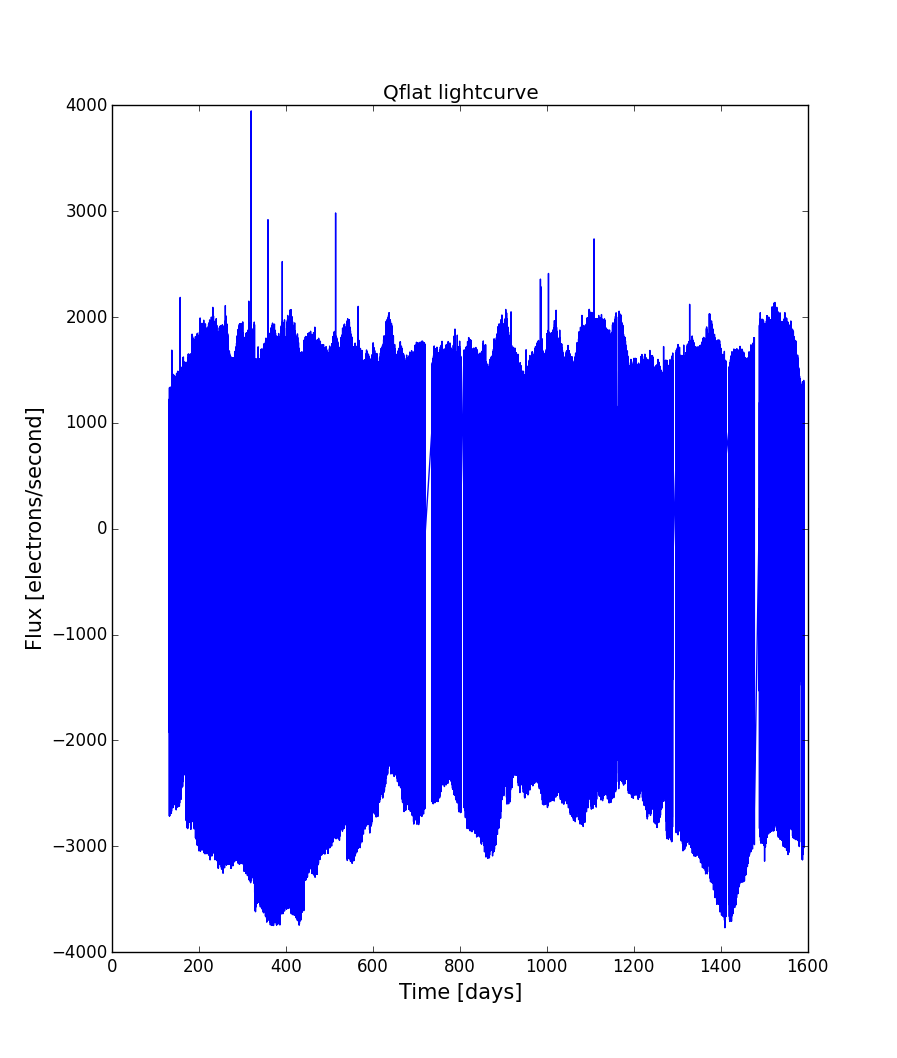
\includegraphics[width=\textwidth]{Qflat_lightcurve.png}
    \caption{The lightcurve after it has been Quarterly-Flatted.}
    \label{fig:Q_lc}
    
\end{figure}

\begin{figure}
    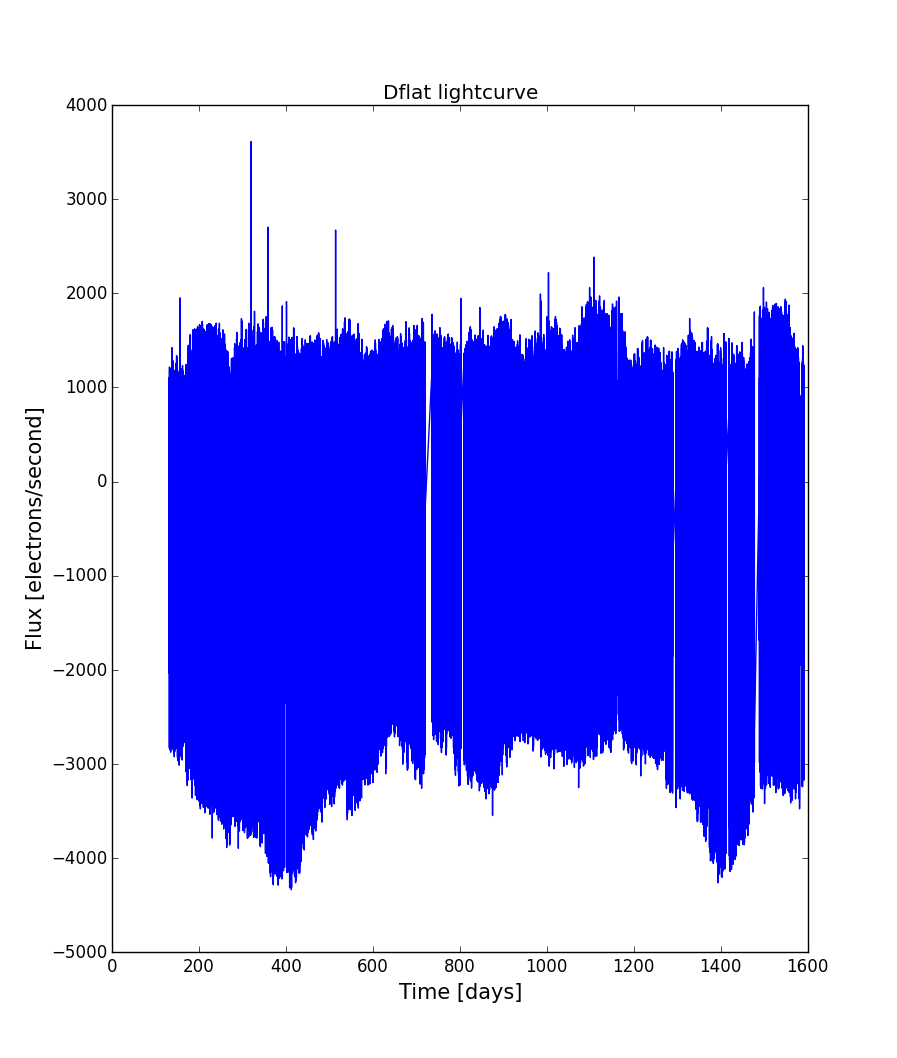
\includegraphics[width=\textwidth]{Dflat_lightcurve.png}
    \caption{The lightcurve after it has been Daily-Flatted.}
    \label{fig:D_lc}
    
\end{figure}

% section Method (end)

\section{Experiments} % (fold)
\label{sec:Experiments}
\subsection{Data Sets} % (fold)
\label{sub:Data Sets}

With its impressive dataset on over 100,000 targets, the \textit{Kepler} data set provides an excellent opportunity to look at stellar variability (the changing of a star's brightness over time).
\textit{Kepler} was designed to be photometrically sensitive, so it is an excellent tool for this purpose.
The time domain nature of the dataset is spectacular, approximately 4~years of data with a 30~minute cadence for each star.
This poses a problem on how to extract features out of the times series data, which we address in Section~\ref{sec:Method}.

The \textit{Galaxy Evolution Explorer} (\textit{GALEX}) is a space telescope that observes in the ultraviolet region of the electromagnetic spectrum.
The ultraviolet emission is often used as an indication of a star's activity.
Stellar activity can be inferred by the presence of starspots on the star's surface.
These are regions where magnetic fields suppress surface convection.

After performing a cross matching of these two data sets, we found 222,158 potential targets.
Not all of these targets have time series data however, so we further pared our data set by limiting it to stars that had lightcurve data.
This resulted in a total of 20,840 stars.
Additional information on our data set is found in Section~\ref{sec:Method}.

% subsection Data Sets (end)

\subsection{Experimental Results} % (fold)
\label{sub:Experimental Results}
As we outlined in the midterm report, our preliminary attempts to cluster the data were not particularly successful.
We first used the K-Means method, but this approach had a few problems.
While the approach can handle large data sets, K-Means only works well when the data can be clustered into a medium number of clusters and if those clusters are very well defined.
Considering the complexity of the physical objects that our data describes, it is easy to see why they would not necessarily fit into well defined clusters.
This could also be partly due to the fact that this preliminary pass did not include time series data, which is an important part of our data set.
The additional features that were acquired from the lightcurves could have made K-Means clustering more effective, but that effectiveness would probably have been marginal.
As can be seen in Figure~\ref{fig:cluster_26_membership}, cluster 4 has an incredibly large population in relation to the rest of the clusters.

\begin{figure}
    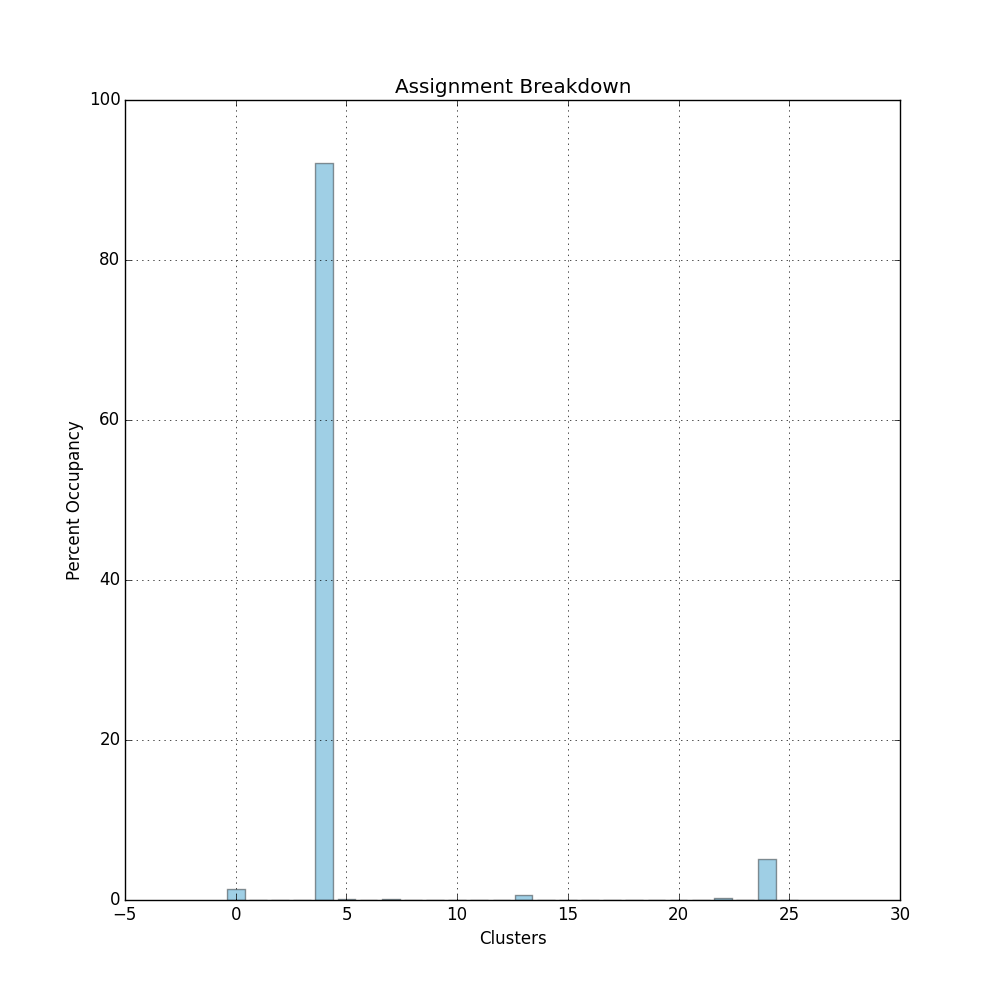
\includegraphics[width=\textwidth]{classBargraph.png}
    \caption{A bar graph illustrating the percent membership breakdown per cluster obtained from K-Means.}
    \label{fig:cluster_26_membership}
    
\end{figure}

After seeing the results of our preliminary clustering attempts we decided to go with hierarchical clustering instead.
Hierarchical clustering is easily able to handle large data sets and large numbers of clusters but the drawback is that it is a computationally expensive method.
We discovered this while attempting to cluster our entire data set.
As a result we decided to first cluster a sample of our data set, which we obtained by taking the square root of the size of our data set, turning it into an integer, and then getting a random permutation, thus picking a sample of size 144 that would be representative of the data set as a whole.

We clustered our sample data set twice, producing dendrograms Figure~\ref{fig:Dend_samp_20} and Figure~\ref{fig:Dend_samp_50}. 
Each of these times represents the number of levels at which we cut off the dendrogram. Figure~\ref{fig:Dend_samp_20} shows the clusters at 20 levels of the hierarchy and Figure~\ref{fig:Dend_samp_50} shows the clusters at 50 levels.

\begin{figure}
    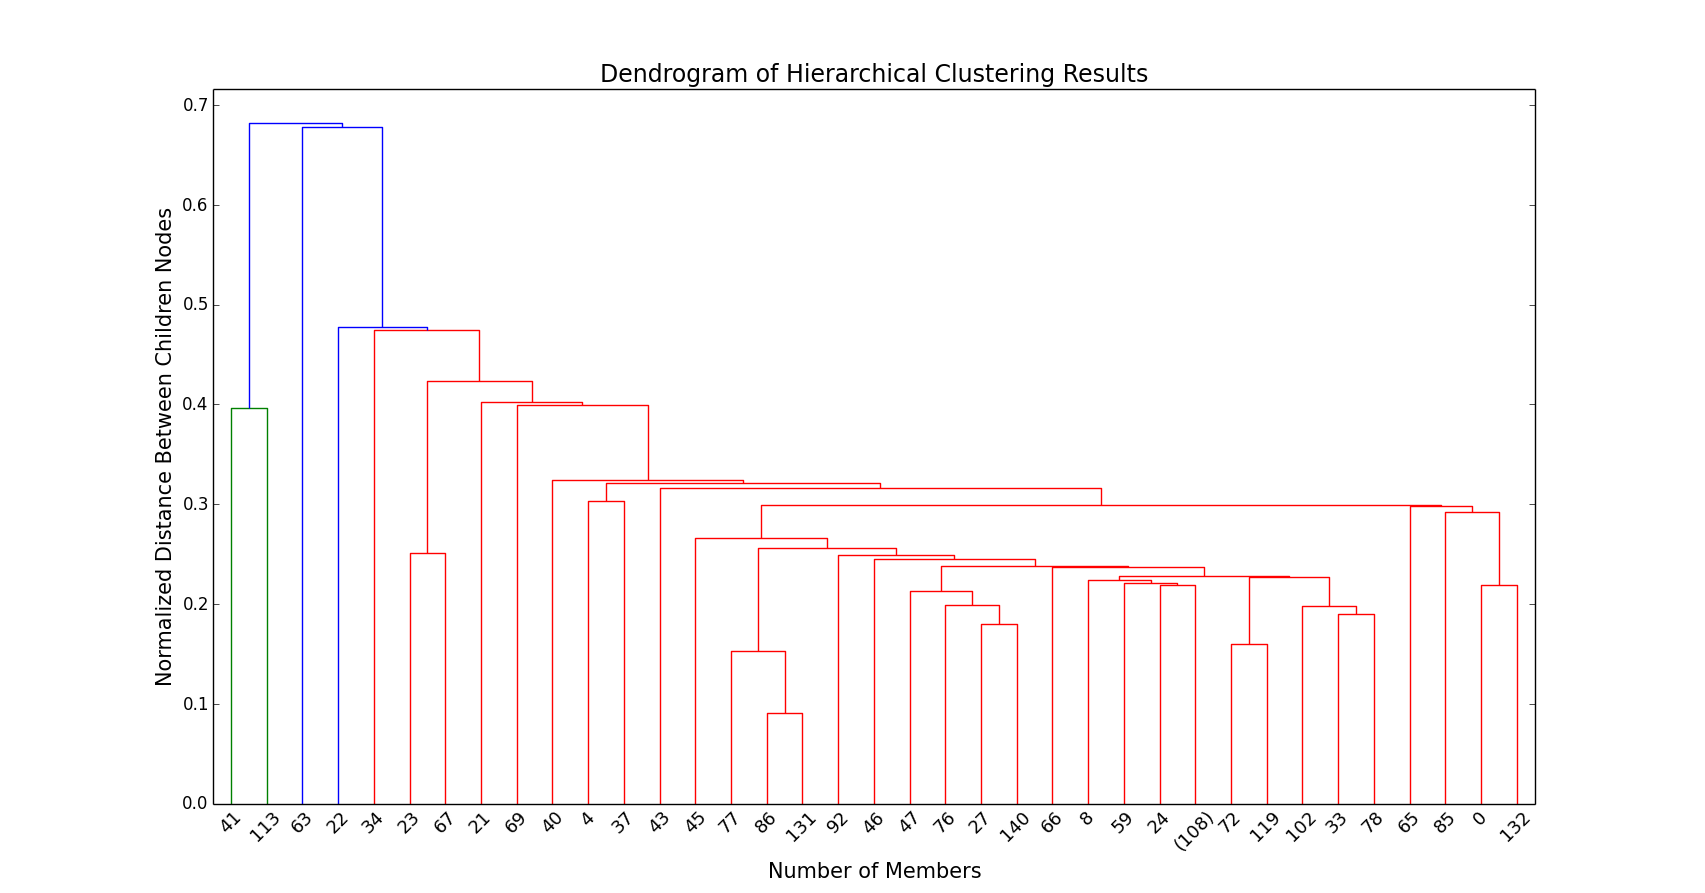
\includegraphics[width=\textwidth]{dend_rand_samp_20_levels.png}
    \caption{A dendrogram of a random sample of our data set, clustered up to 20 levels.}
    \label{fig:Dend_samp_20}
    
\end{figure}

\begin{figure}
    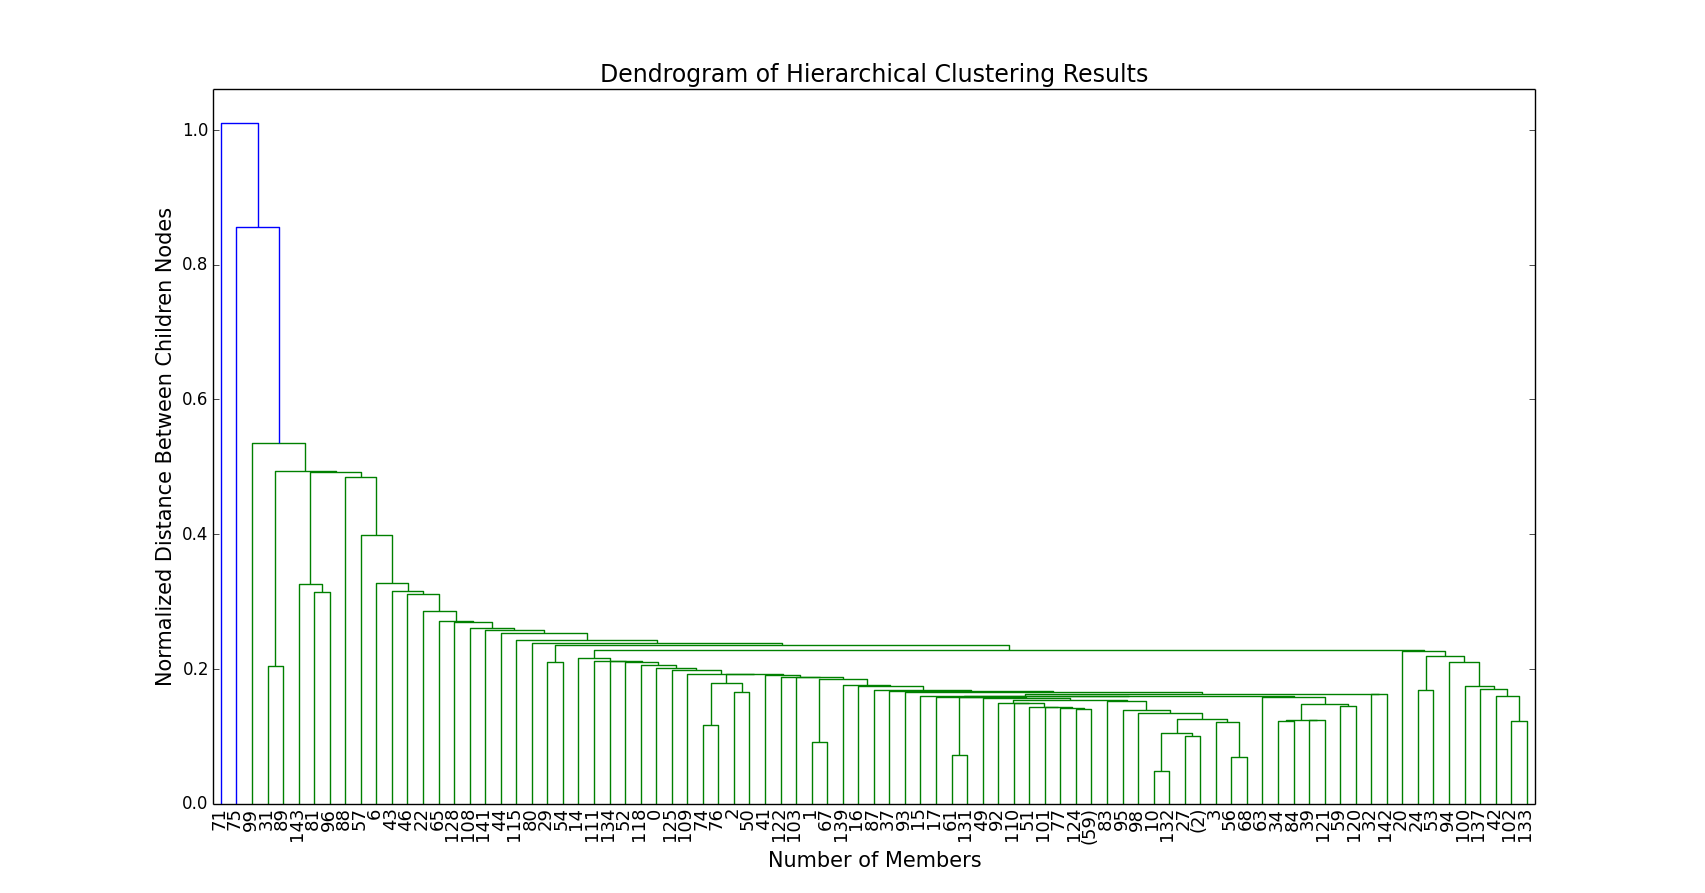
\includegraphics[width=\textwidth]{dend_pop_samp.png}
    \caption{A dendrogram of a random sample of our data set, clustered up to 50 levels.}
    \label{fig:Dend_samp_50}
    
\end{figure}

We also managed to cluster our entire data set.
The process took several hours and the resulting dendrogram, clustered up to 50 levels, can be seen in Figure~\ref{fig:Dend_all_50}.

\begin{figure}
    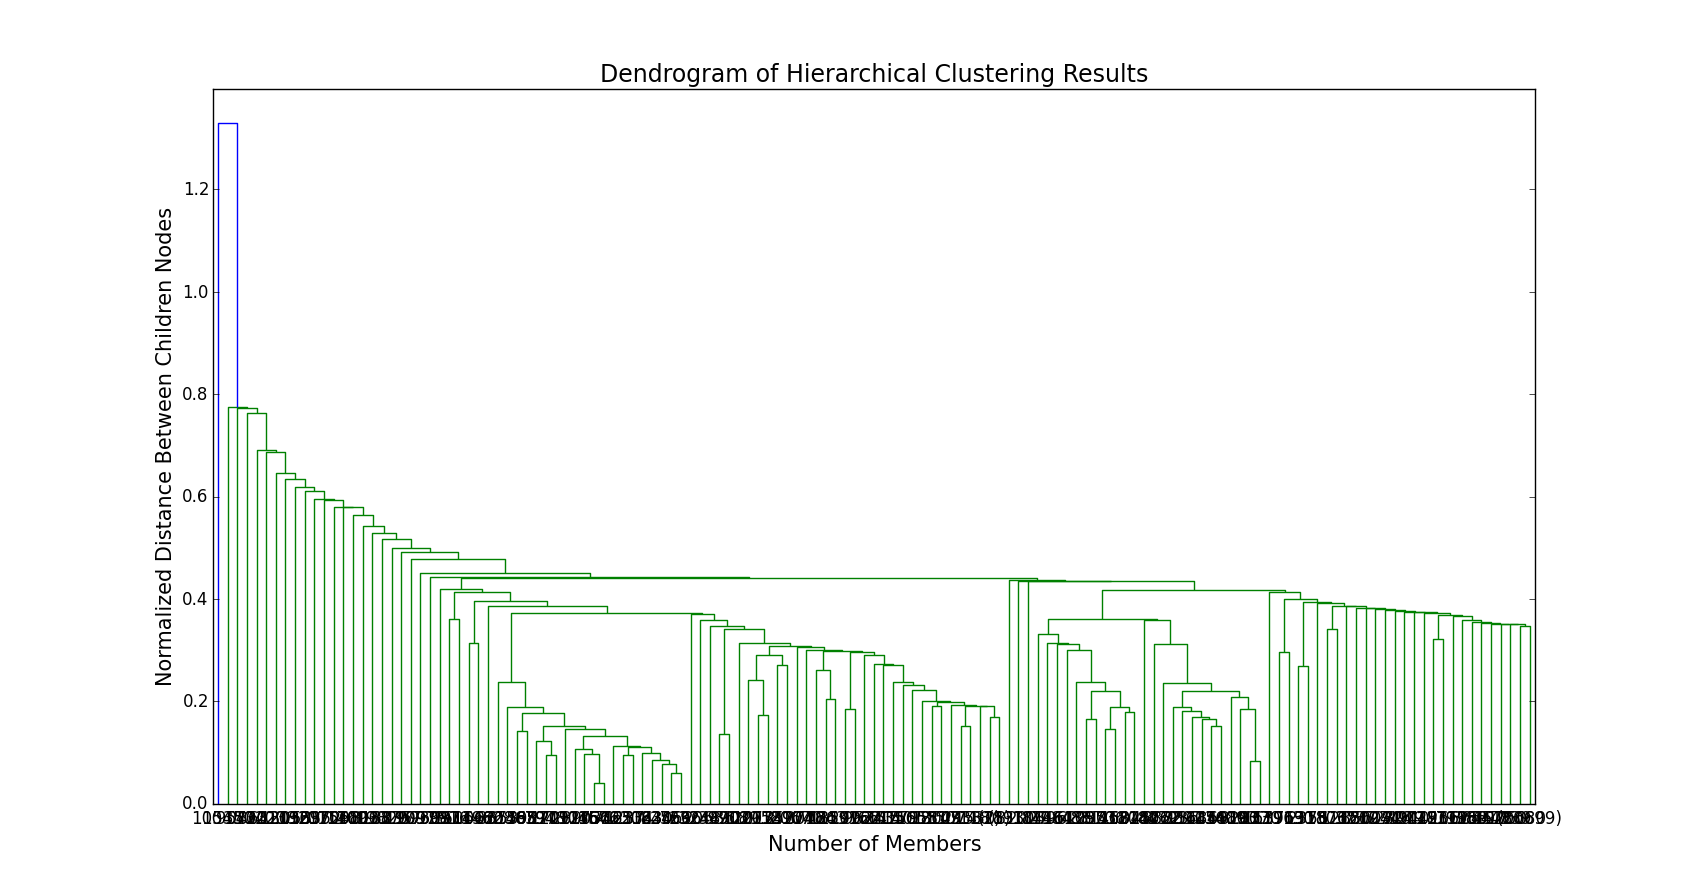
\includegraphics[width=\textwidth]{dend_50_full.png}
    \caption{A dendrogram of our entire data set, clustered up to 50 levels.}
    \label{fig:Dend_all_50}
    
\end{figure}

In all of our dendrograms one can see a large U bar in the middle of the figure.
This is particularly interesting, as it indicates that a large number of clusters can trace their lineage back to a few select overarching clusters.
On the leftmost side of our figures there is a small group of clusters that breaks off quite early.
This indicates that these groups of stars are particularly distinct from the rest and the clusters that contain them should be fairly homogeneous. 

Overall hierarchical clustering seems to perform better than K-Means.
As can be seen from Figure~\ref{fig:Bar_Samp}, the membership of the clusters is much more evenly spread for hierarchical clustering than for K-Means.
Considering that we have more features for this final clustering method than we did for our preliminary pass (at the time we had not yet implemented our time series processing), this seems a good indication that hierarchical is the superior method in this case.

\begin{figure}
    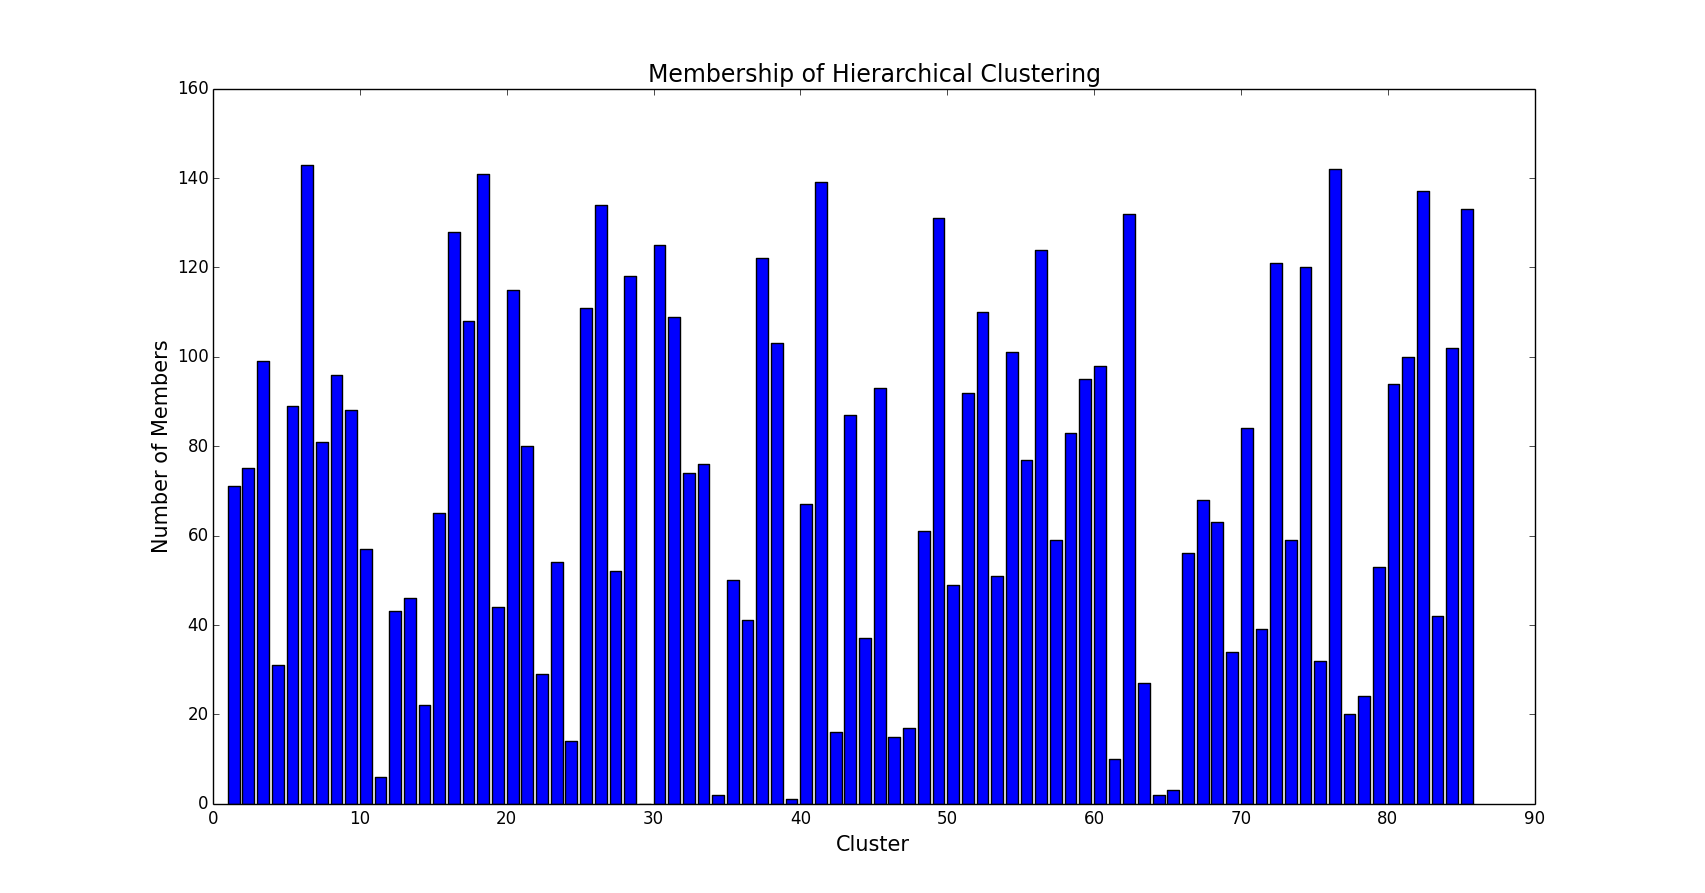
\includegraphics[width=\textwidth]{bar_pop_samp.png}
    \caption{A bar graph of a sample of our data, showing the number of members in each cluster.}
    \label{fig:Bar_Samp}
    
\end{figure}


Because of the large data set size we expected that the stars would be clustered fairly evenly, so our final method, hierarchical, seems to be a much better method to use for this problem.
We must also consider the type of objects that we are working with.
Some types of stars have wildly distinct behavior and so, for example, the features we extracted from their lightcurves would almost immediately identify them as one particular group that belongs in a separate cluster.
If our data set had been comprised of just these kinds of stars then K-Means would have been a good method to use since the resulting clusters would no doubt have been very distinct and easy to separate.
Our real data set, however, also included stars that were perhaps not so distinguishable from one another.
In fact, these are the kinds of stars that were in the majority, so the potential overlap for clusters for these types of stars is great, meaning that our clustering method would need to be able to handle potential overlap.
Hierarchical seemed to be up to the challenge and greatly exceeded the performance of K-Means.
% subsection Experimental Results (end)
% section Experiments (end)


\section{Summary} % (fold)
\label{sec:Summary}
Our research problem involved taking an incredibly large astronomical data set, which included time series lightcurves, and clustering the stellar objects it described.
The first clustering method that we attempted was K-Means clustering which performed poorly on our data set.
The final method we chose was hierarchical clustering, which performed much better than K-Means.

In Section~\ref{sec:Related Work}, we discussed literature that pertained to distributed data mining.
We did not use this approach for the actual clustering of our data, but we did apply its principles to the data preprocessing.
Preprocessing the data took the longest time of any step of our data analysis, but we were able to mitigate the issue by making our preprocessing distributed.
This is discussed in further detail in Section~\ref{sec:Method}.
The challenge with using distributed clustering is that it would be difficult to implement with certain types of algorithms.
Since distributed clustering relies on finding local representatives that are then sent to a global site and clustered again, a method like K-Means would be less challenging to implement than hierarchical clustering.

We have learned a lot in the making of this project.
The first thing is that we learned more about the Julia language, which we used almost exclusively.
While similar to Python, Julia has many different features and has proved overall to be a better language for the processing of scientific data.
We also learned a lot about how to handle large amounts data and how to write code to accommodate it.
The great majority of our time was spent on writing code to preprocess our data and including safeguards so that should our program crash, we would be able to continue right where we left off.

A potential line of inquiry for the future could be to make distributed clustering work for hierarchical clustering.
In addition, in the future we might try accuracy testing based on a small, labeled subset of the data set we used for this project.
Other potential work could include implementing other types of clustering methods in order to compare their performance.
Also, analyzing tight clusters and potentially classifying them.

% section Summary (end)


\newpage
\section{Group Contribution} % (fold)
\label{sec:Group Contribution}
Both group members contributed fairly equally to this project.
While Mark contributed more of the astronomical knowledge and took the lead of data acquisition and preprocessing, Vera took the lead on the clustering of the data.
% section Group Contribution (end)

\newpage
\bibliographystyle{plainnat}
\bibliography{sources}
\end{document}
